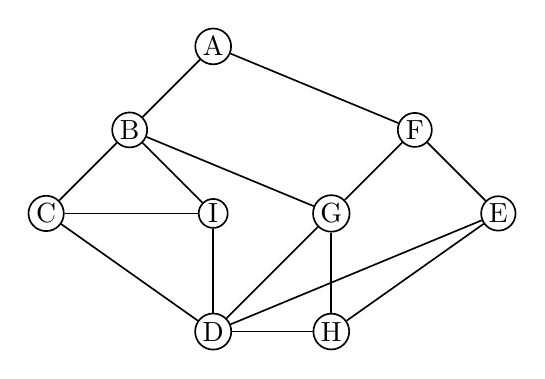
\begin{tikzpicture}[scale=0.25,node distance=1.5cm,semithick,inner sep=1pt,bend angle=45]
%\draw[help lines] (-3,-3) grid (3,0);
\node[circle,draw]   (A)                    {\tf A};
\node[]   (A1)[right of=A]       {};
\node[circle,draw]   (B) [below left  of=A] {\tf B};
\node[circle,draw]   (F) [below right of=A1]{\tf F};
\node[circle,draw]   (C) [below left  of=B] {\tf C};
\node[circle,draw]   (G) [below left  of=F] {\tf G};
\node[circle,draw]   (E) [below right of=F] {\tf E};
\node[circle,draw]   (H) [below       of=G] {\tf H};
\node[circle,draw]   (I) [below right of=B] {\tf I};
\node[circle,draw]   (D) [below       of=I] {\tf D};
                                              
\path
(A) edge node{} (B)
    edge node{} (F)
(B) edge node{} (C)
    edge node{} (G)
    edge node{} (I)
(F) edge node{} (G)
    edge node{} (E)
(C) edge node{} (I)
    edge node{} (D)
(G) edge node{} (H)
    edge node{} (D)
(E) edge node{} (H)
    edge node{} (D)
(H) edge node{} (D)
(I) edge node{} (D);                     
\end{tikzpicture}
